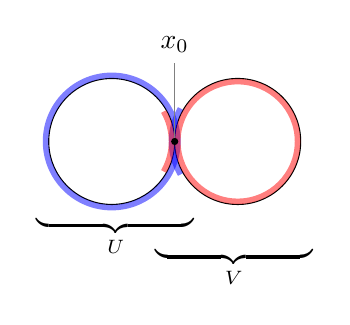
\begin{tikzpicture}
\draw (-0.8,0) circle (0.8);
\draw (0.8,0) circle (0.8);
\draw[blue, line width=2pt, opacity=0.5] (-0.8,0) circle (0.84);
\draw[blue, line width=2pt, opacity=0.5] (0.8,0) ++(150:0.84) arc (150:210:0.84);
\draw[red, line width=2pt, opacity=0.5] (0.8,0) circle (0.76);
\draw[red, line width=2pt, opacity=0.5] (-0.8,0) ++(-30:0.76) arc (-30:30:0.76);
\fill (0,0) circle (1.3pt);
\draw[gray] (0,0.05) -- (0,1.0);
\node[above] at (0,1.0) {$x_0$};
\node at (-0.75,-1.2) {$\underbrace{\hspace{2cm}}_{U}$};
\node at (0.75,-1.6) {$\underbrace{\hspace{2cm}}_{V}$};
\end{tikzpicture}
